\begin{figure}[hbtp]
  \centering
  \subfigure{
    \label{fig:about-pruning--all}
    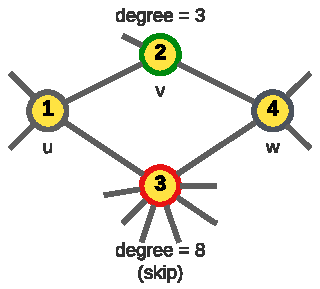
\includegraphics[width=0.38\linewidth]{out/about-pruning.pdf}
  } \\[-2ex]
  \caption{Low degree vertices, such as $2$, confer significant similarity among its neighbors, while high-degree vertices, such as $3$, do not. Here $4$ is a second-order neighbor of $1$.}
  \label{fig:about-pruning}
\end{figure}
